\documentclass[tikz, preview]{standalone}

\usepackage{amsfonts, amsthm, amssymb, amsmath, stmaryrd, etoolbox}
\usepackage{tikz}
\usetikzlibrary{matrix,arrows}

\begin{document}
\[
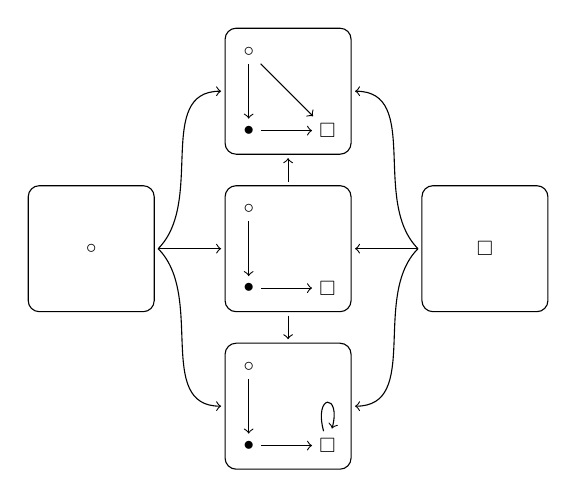
\begin{tikzpicture}
\draw[rounded corners] (1.7,-0.3) rectangle (3.3,1.3);
\draw[rounded corners] (1.7,1.7) rectangle (3.3,3.3);
\draw[rounded corners] (1.7,3.7) rectangle (3.3,5.3);
\draw[rounded corners] (-0.8,1.7) rectangle (0.8,3.3);
\draw[rounded corners] (4.2,1.7) rectangle (5.8,3.3);
%
\node[scale=0.75] (ai) at (0,2.5) {$\circ$};
\node[scale=0.75] (co) at (5,2.5) {$\square$};
\node[scale=0.75] (a1) at (2,5) {$\circ$};
\node[scale=0.75] (b1) at (2,4) {$\bullet$};
\node[scale=0.75] (c1) at (3,4) {$\square$};
\node[scale=0.75] (a2) at (2,3) {$\circ$};
\node[scale=0.75] (b2) at (2,2) {$\bullet$};
\node[scale=0.75] (c2) at (3,2) {$\square$};
\node[scale=0.75] (a3) at (2,1) {$\circ$};
\node[scale=0.75] (b3) at (2,0) {$\bullet$};
\node[scale=0.75] (c3) at (3,0) {$\square$};
%
\draw [->] (a1) edge (b1);
\draw [->] (b1) edge (c1);
\draw [->] (a2) edge (b2);
\draw [->] (b2) edge (c2);
\draw [->] (a3) edge (b3);
\draw [->] (b3) edge (c3);
\draw [->] (a1) edge (c1);
\draw [->] (c3) edge [loop above] (c3);
%
\path [->] (0.85,2.5) edge[out=0,in=180] (1.65,2.5);
\path [->] (0.85,2.5) edge[out=45,in=180] (1.65,4.5);
\path [->] (0.85,2.5) edge[out=-45,in=180] (1.65,0.5);
\path [->] (4.15,2.5) edge[out=180,in=0] (3.35,2.5);
\path [->] (4.15,2.5) edge[out=135,in=0] (3.35,4.5);
\path [->] (4.15,2.5) edge[out=225,in=0] (3.35,0.5);
\draw [->] (2.5,3.35) -- (2.5,3.65);
\draw [->] (2.5,1.65) -- (2.5,1.35);
\end{tikzpicture}
\]
\end{document}
